\documentclass[12pt, letterpaper, titlepage, hidelinks]{article}

% Packages
\usepackage[letterpaper, margin=1in]{geometry}
\usepackage[utf8]{inputenc}
\usepackage{fancyhdr}
\usepackage{setspace}
\usepackage{amssymb}
\usepackage{amsmath}
\usepackage{multirow}
\usepackage{array}
\usepackage{graphicx}
\usepackage{tabularx}
\usepackage{booktabs}
\usepackage{hyperref}
\usepackage{scrextend}
\usepackage{verbatim}
\usepackage[english]{babel}
\usepackage{blindtext}
\usepackage{capt-of}
\usepackage{float}
\usepackage{caption}
\usepackage{apacite}
\usepackage{mathrsfs}
\usepackage{pdfpages}
\usepackage[autostyle, english = american]{csquotes}
\MakeOuterQuote{"}

\graphicspath{ {Images/} }


\newenvironment{nospaceflalign*}
{\setlength{\abovedisplayskip}{0px}\setlength{\belowdisplayskip}{0px}%
	\csname flalign*\endcsname}
{\csname endflalign*\endcsname\ignorespacesafterend}

% Title Page
\title{4DM4 Assignment 1 \\ RISC Scheduling of the Chacha20 Stream Cipher}
\author{Ashpan Raskar raskara 400185326\\
		Ahnaf Bhuiyan bhuiya3 400198359}
\date{\today}



\begin{document}

\maketitle
\tableofcontents
\newpage
\setlength{\parindent}{0pt}
\setcounter{secnumdepth}{0}
\section{Part A}
	\subsection{A1}
		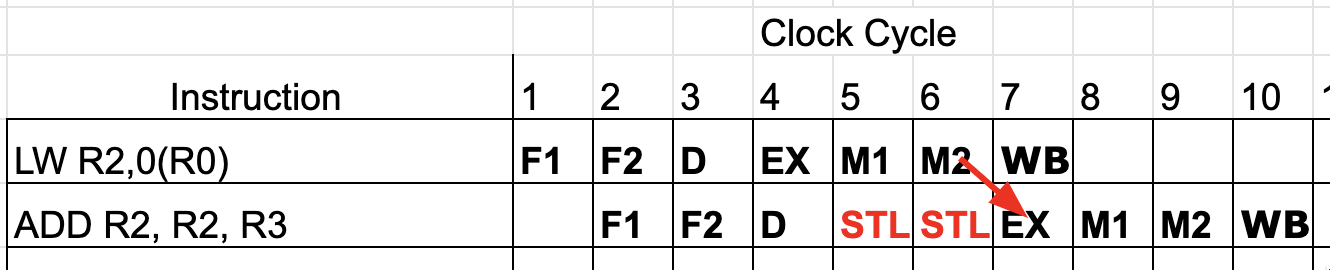
\includegraphics[width=\textwidth]{A1}
	\subsection{A2}
	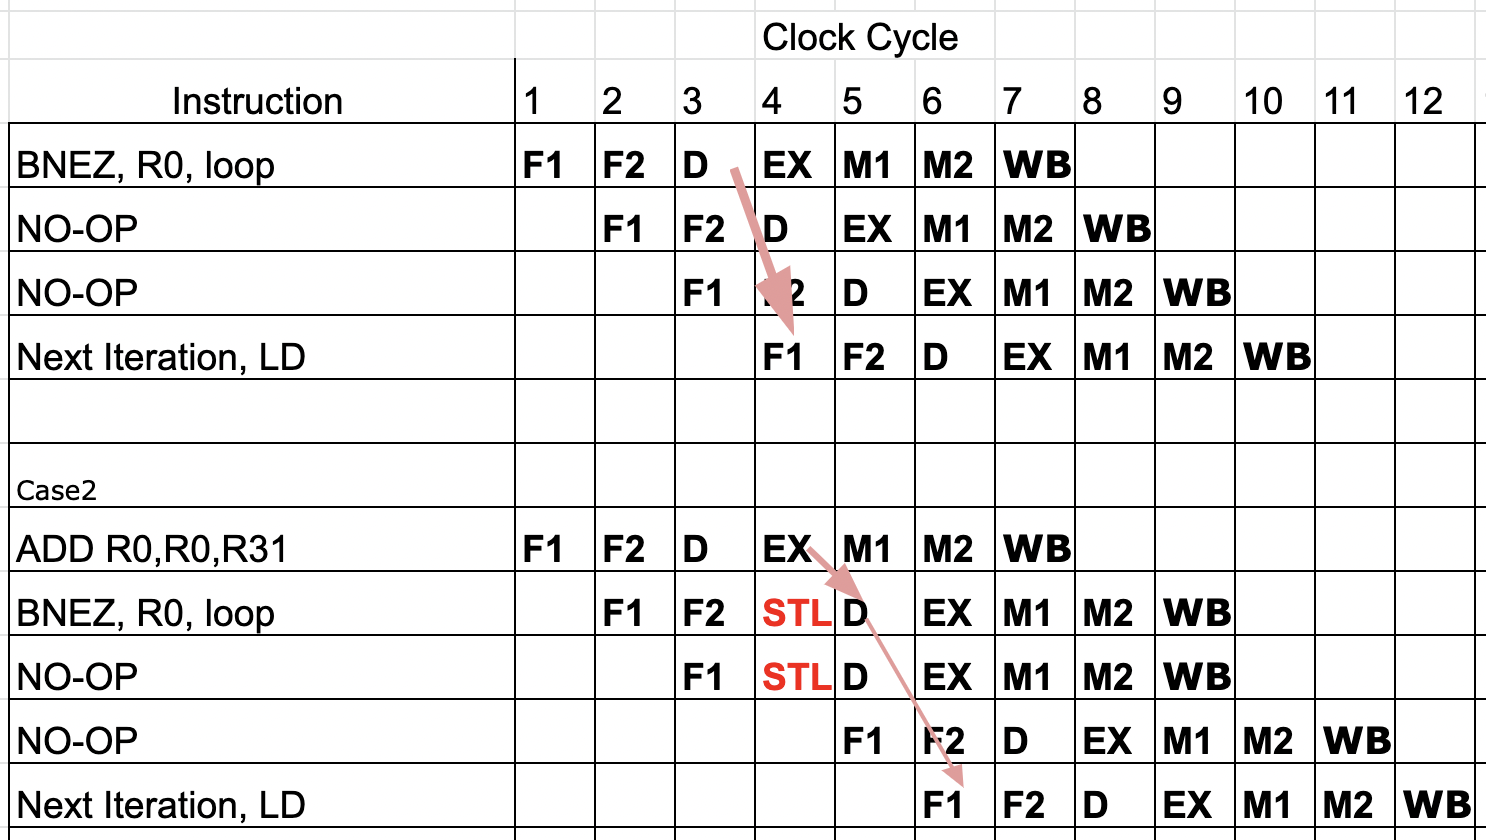
\includegraphics[width=\textwidth]{A2}
\section{Part B}
	\subsection{B1}
		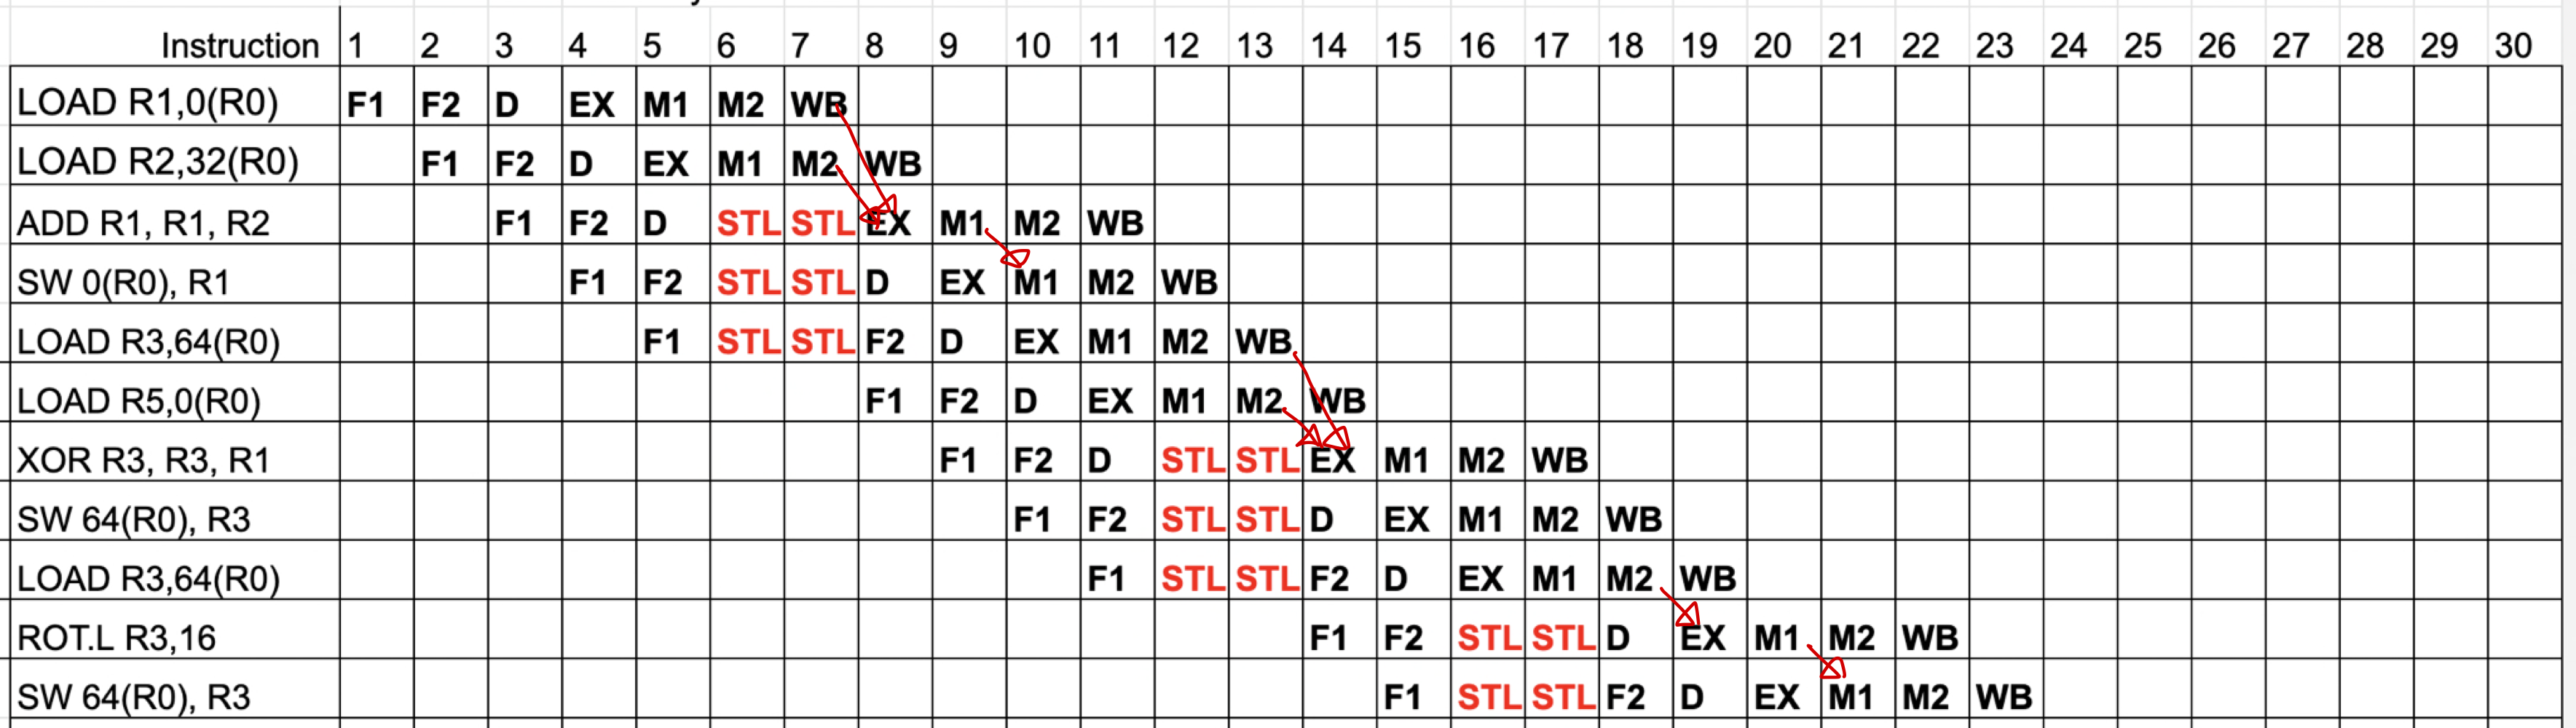
\includegraphics[width=\textwidth]{B1}
	\subsection{B2}

	\subsection{B3}
		It takes \textbf{92 clock cycles} to complete the quarter round operation of the Chacha20 stream cipher. The number of clock cycles is calculated by adding the number of clock cycles required to complete each of the four operations in the quarter round.
	\subsection{B4}

	\subsection{B5}

	\subsection{B6}

	\subsection{B7}
	% 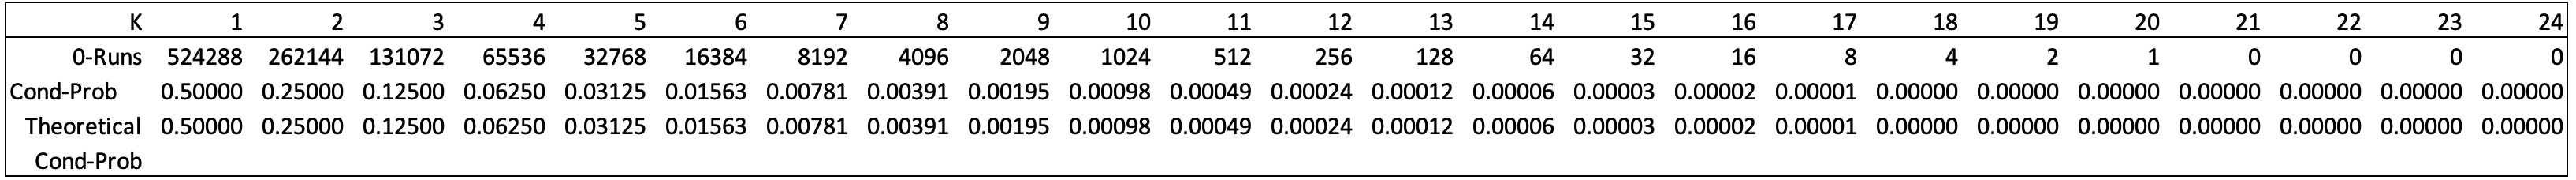
\includegraphics[width=\textwidth]{0_run_table}
\end{document}          